%!TEX root = ../main.tex
\section{Modelling a DC motor}
This section deals with the modelling and parameterisation of a brushed DC motor, specifically the Pittmann 9234 24V servomotor.
Figure \ref{fig:dcmotormodel} is a simple model of a DC motor.
The parameters of this model will be estimated by experimentation.

\begin{figure}[!h]
	\centering
	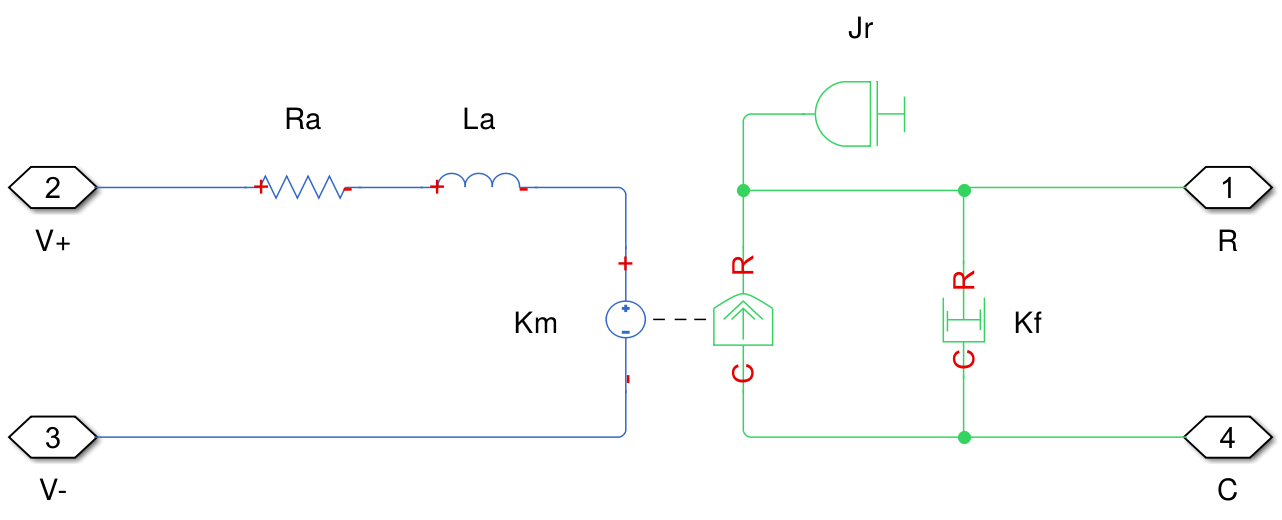
\includegraphics[width=\linewidth]{graphics/dcmotormodel.png}
	\caption{Simulink model of a brushed DC motor.}
	\label{fig:dcmotormodel}
\end{figure}


\subsection{Armature Resistance - $R_a$}
The armature resistance, $R_a$ in figure \ref{fig:dcmotormodel}, can be found simply by applying Ohm's law.
The current through a resistor is well defined when a voltage is applied across it.

\begin{figure}[!h]
	\centering
	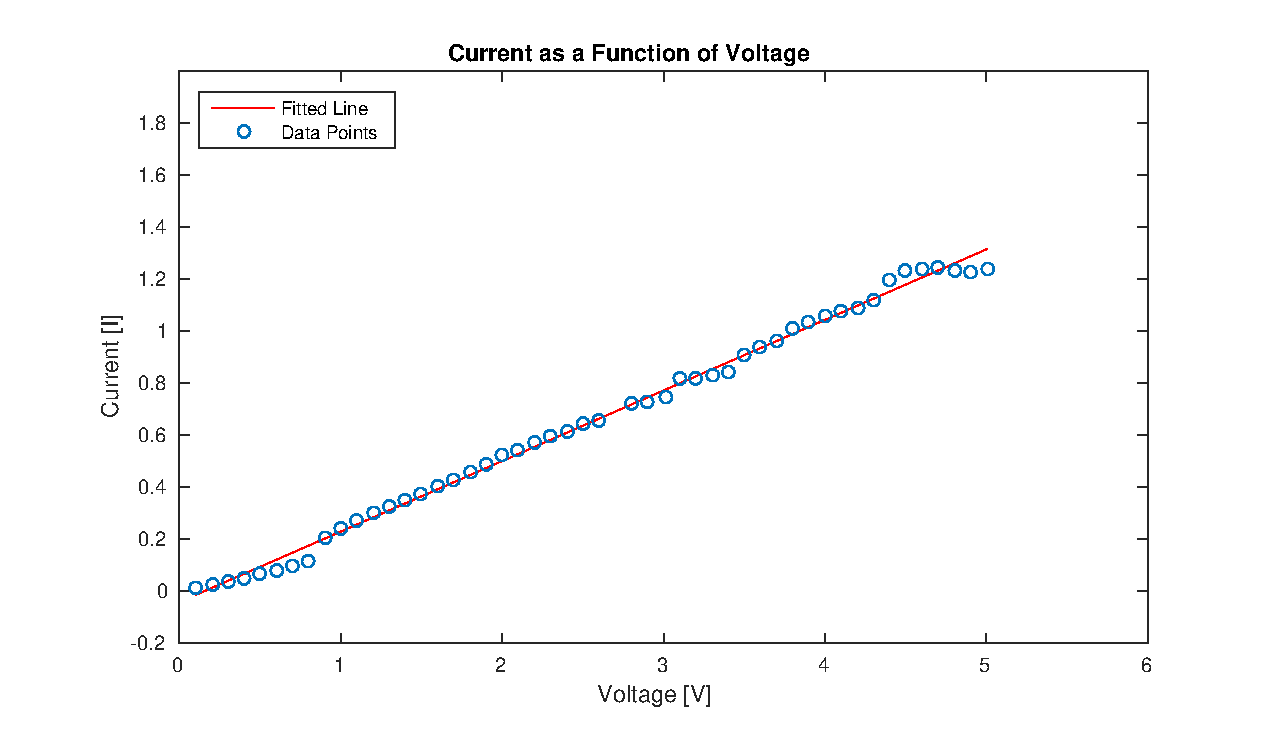
\includegraphics[width=\linewidth]{graphics/raplot}
	\caption{Current as a function of voltage with the rotor blocked.}
	\label{fig:raplot}
\end{figure}

However, when the rotor is spinning, the circuit produces back-EMF.
This counters the input voltage, effectively lowering the current through $R_a$.
In order to avoid this effect the rotor is blocked.
Since, with a blocked rotor, there will be no change in voltage in the system, the inductor acts as a short circuit, reducing the circuit to a voltage across a resistor. 

Figure \ref{fig:raplot} shows the data collected in order to determine the value of the armature resistance.
A voltage is applied across the terminals at 0.5 V.
According to the datasheet \cite{pittmann} the current at maximum allowed continuous torque is 1.75 A.
This current is reached at 5 V, therefore, the measurements stop there.
As can be seen from the figure, a line is fitted to the data.
This is done using the linear least squares method with the following result:
$$I(V)=0.331\cdot V-0.138$$
with $R^2=0.994$.
Since for the plot $I(V)$:
$$R_a = \frac{1}{\text{slope}} = 3.02\Omega$$
However, at $I(0)$ the model will result in a small negative current.
This is obviously not correct; no current would be expected at zero voltage.
Adjusting the model such that it will intersect the origin results in a higher resistance of $R_a=3.43\Omega$.
